  \section{Results}
\label{sec:results}

Next, we present the results of PARSEC simulation cycles on the proposed coded model and a baseline model. The goal is to simulate the benefits of improved read accesses, which bounds the amount of improvement we can expect in a full hardware implementation. Encoding and decoding can be done offline in parallel and is therefore ignored. We also consider the delays of parity bank writebacks to be negligible. The coded model was evaluated with the following reorder buffer sizes: $\{8,32,128,1024\}$. For some simulation, we also evaluated the coded model's performance with additional reorder buffer sizes: $\{1, 16\}$.
\subsection{Cycle Simulation Results}
\label{sec:results}

The proposed coded system performs consistently well across the PARSEC 2.1v and 3.0v benchmarks. We find that the parity structure has a small impact on the performance of the system, and the reorder buffer length is  the largest factor in the efficacy of the system. For several scenarios we show greater than 50\% reduction in the number of CPU cycles needed for the simulation to complete. In the figures below we show the number of simulated CPU cycles for the proposed coded system compared to the number of simulated CPU cycles for the baseline coded system. Most notable in these results is that a short reorder buffer length of 8 is sufficient to achieve significant improvement, and once the reorder buffer reaches a certain length the marginal benefits of increasing the length of the buffer diminish.

We simulated four different parity architectures. First, we simulate parity banks with symbols composed from four data bank symbols. We simulate the architecture pictured in Figure~\ref{fig:memsys} and the architecture which only contains P0 through P3. Next, we simulate the parity banks as mere duplicates of the data banks. Finally, we simulate the parity banks with symbols composed from two data banks. We use 12 parity banks in this architecture. 


\begin{figure}[h!]
		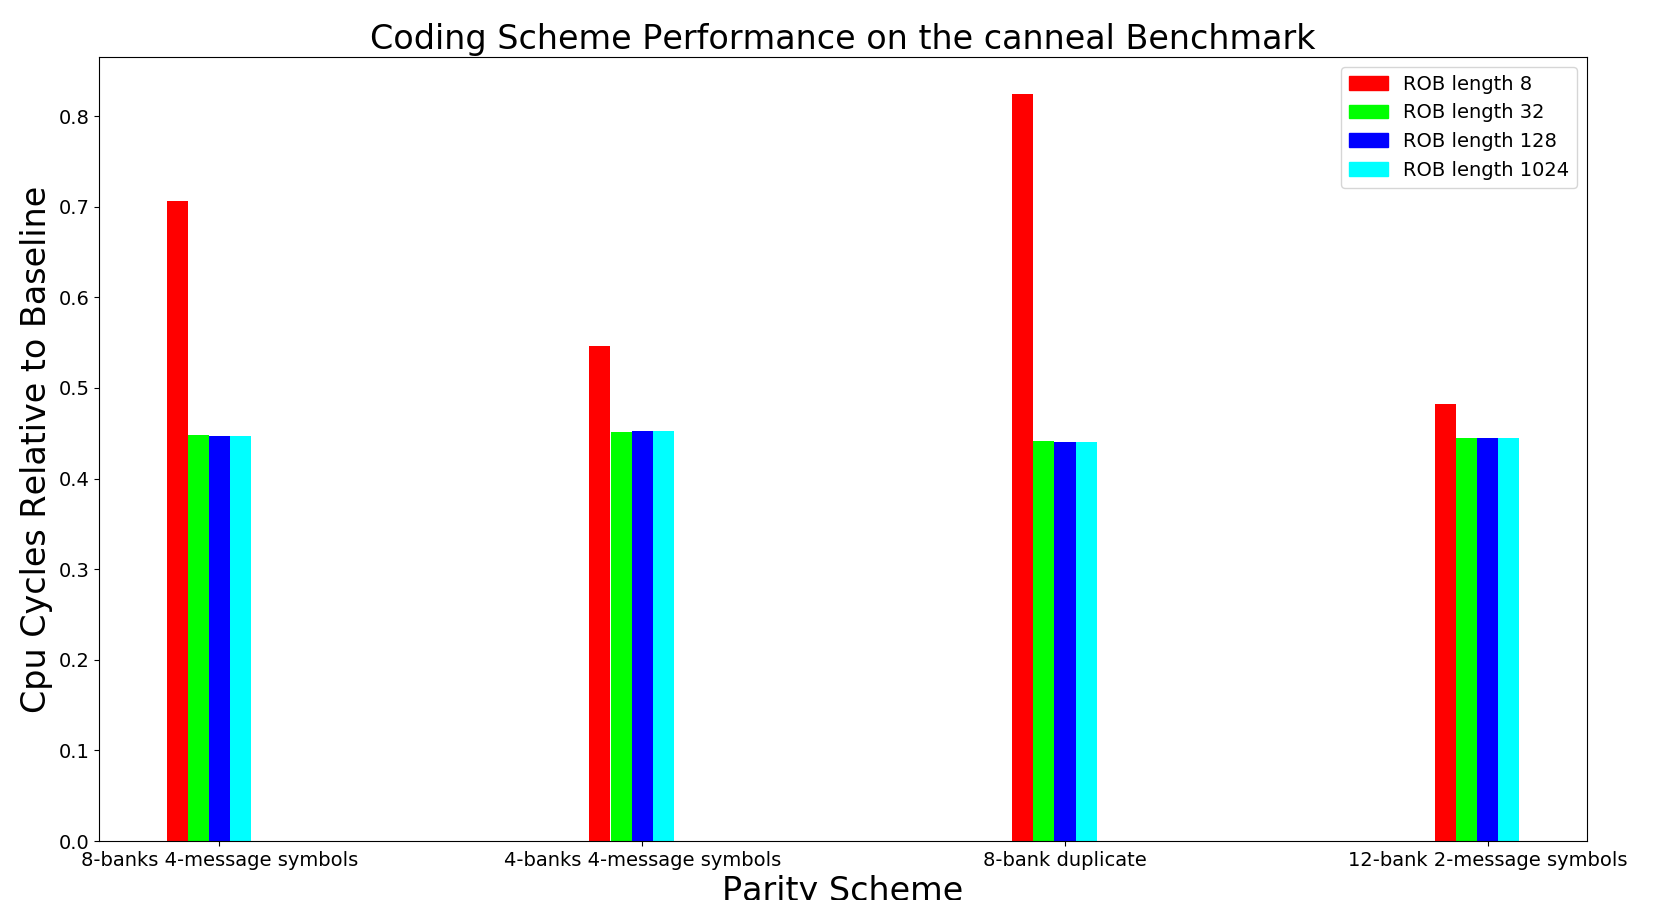
\includegraphics[width=\linewidth]{figures/canneal_results.png}
		\caption{The results of running the 8-core Canneal memory trace through Ramulator}
		\label{fig:canneal_results}
\end{figure}
		

\subsection{Augmented PARSEC Results}
\label{sec:aug_results}

The augmentations on the PARSEC traces significantly impacts how the proposed coded system performs. Figure~\ref{fig:vips_split_results} shows the simulation results for the vips benchmark with the increased number of bands. The figure shows that the proposed coded system is able to achieve improvements similar to those picture in Figure~\ref{fig:canneal_results}, however a larger reorder buffer length is needed to achieve these results. Figure~\ref{fig:vips_ramp} shows the simulation results for the vips benchmark with the ramped memory accesses. Again, we see that the a larger reorder buffer length is needed to maximize the performance of the system. We also observe that here, for small reorder buffer sizes, the proposed memory system performs worse than baseline. The reason for this is that the amount of memory used for dynamic coding is too small for the ramp memory augmentation. Increasing the memory allocated to dynamic coding results in improved performance, as seen in Figure \#\# \Matt{TODO}.

\begin{figure}[h!]
		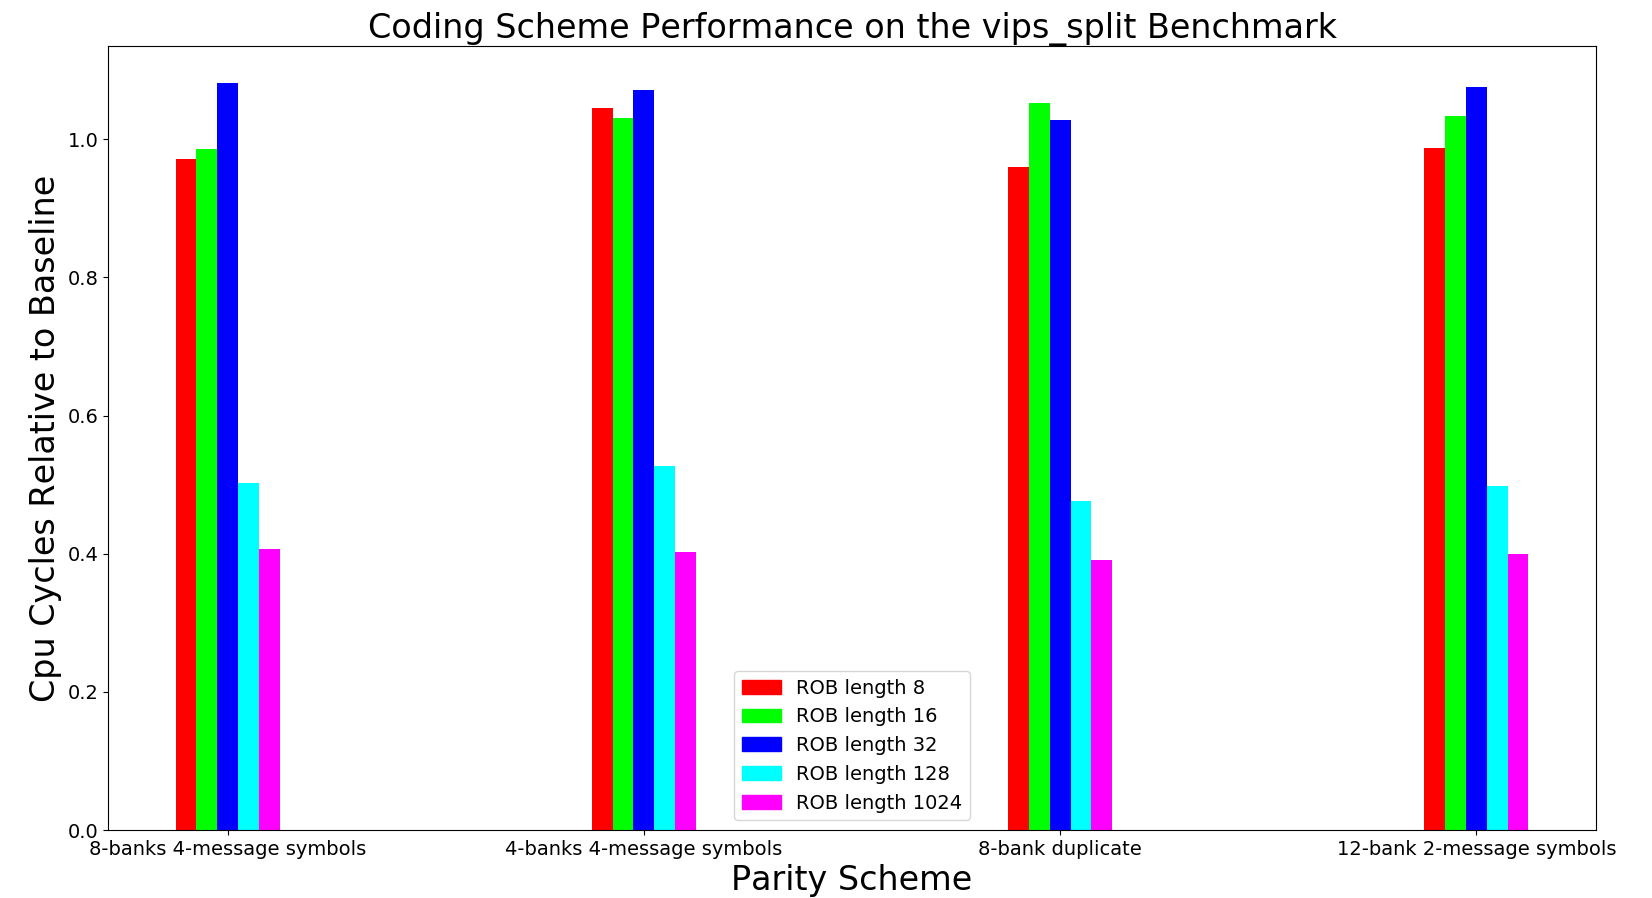
\includegraphics[width=\linewidth]{figures/vips_split_results.png}
		\caption{The performance of the proposed coded system on the trace pictured in Figure~\ref{fig:vips_split} \Matt{TODO: This image should be replaced with one for a simulation that uses a large dynamic coding region}}
		\label{fig:vips_split_results}
\end{figure}


\begin{figure}[h!]
		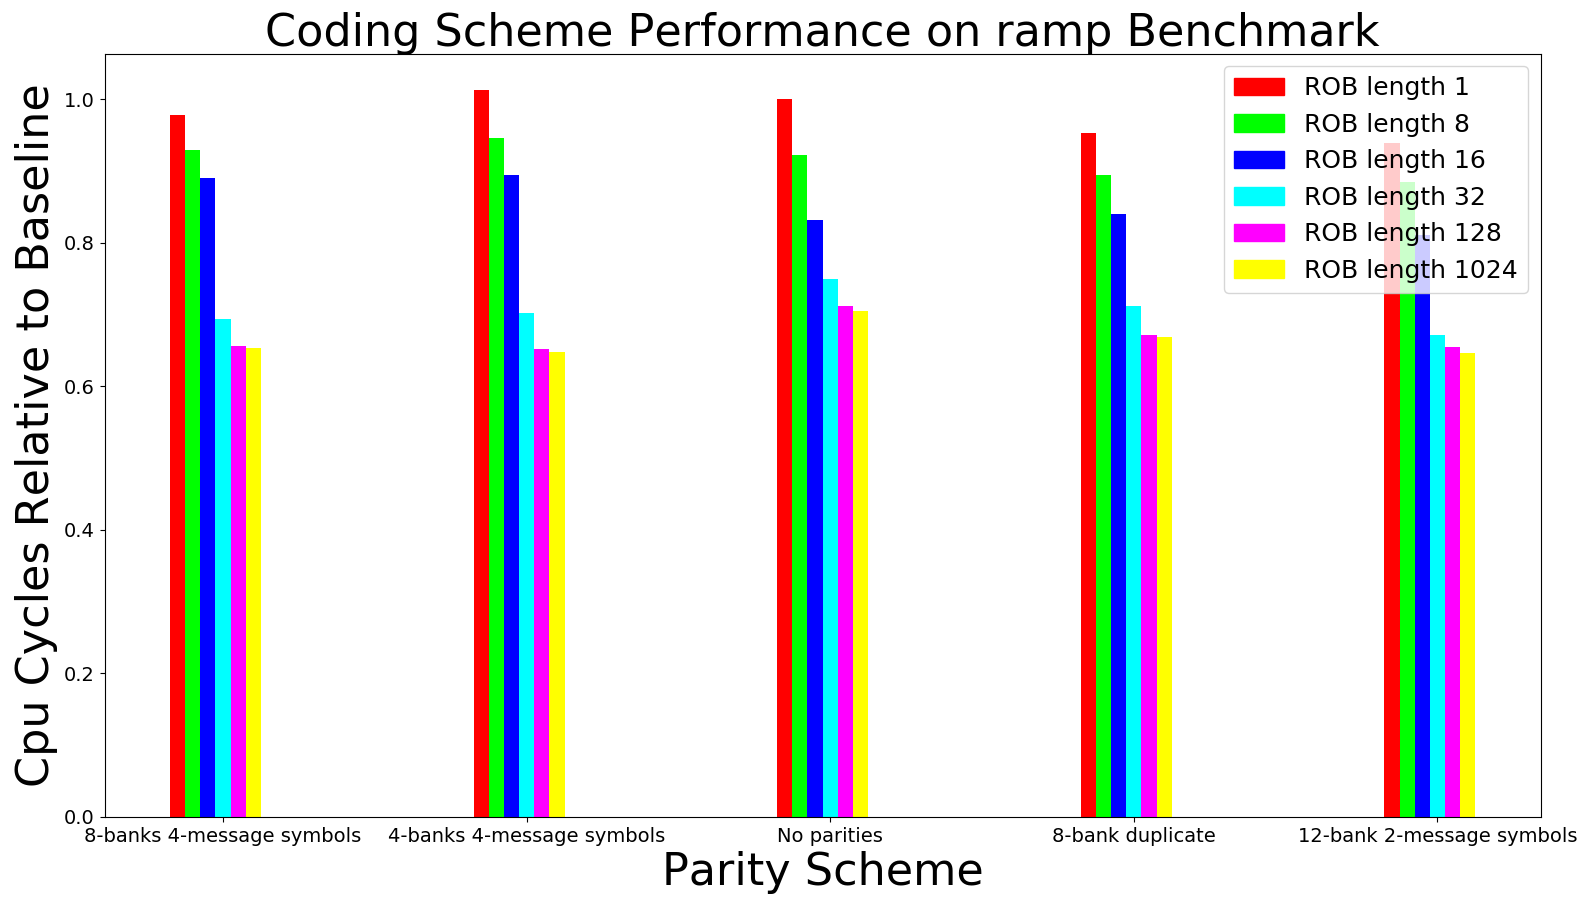
\includegraphics[width=\linewidth]{figures/vips_ramp_results.png}
		\caption{The performance of the proposed coded system on the trace pictured in Figure~\ref{fig:vips_ramp}}
		\label{fig:vips_ramp_results}
\end{figure}